\title{A short report on: \\Transcription Factor Activity of C. Elegans}
\author{
        Muhammad Arifur Rahman \\
        Department of Computer Science\\
        The University of Sheffield\\ Sheffield, UK\\
}
\date{\today}

%\documentclass[12pt]{article}

\documentclass[a4paper,10pt]{report}
\usepackage[utf8]{inputenc}

\usepackage{graphicx} % Allows including images
\usepackage{booktabs} % Allows the use of \toprule, \midrule and \bottomrule in tables
\usepackage{epstopdf} % Allows to view .eps files
\usepackage{amsmath}
\usepackage{amssymb}
\usepackage{color}
\usepackage{url}


\begin{document}
\maketitle

%\begin{abstract}
%This is the paper's abstract \ldots
%\end{abstract}

\section{Motivation}
	\begin{itemize}
	  \item Caenorhabditis Elegans, a saprophytic nematode is an inhabitant of soil and leaf-litter and found 
		in most of the parts of the world~\cite{hope}.
	  \item Scientific reports on C.Elegans appeared in the literature for more than 100 years.
	  \item After the genetics paper of Brenner's ~\cite{brenner} C. Elegans emerged as an important experimental model.
	  \item Based on the bioinformatics approach used C. Elegans is 60-80\% homologies with human genes. ~\cite{kaletta}.
	  \item Within a very short period of time (approximately 3days) allows a large-scale (300+ of offspring) production ~\cite{hope}. 
	  \item In molecular biology and genetics, a transcription factor is a protein that binds to specific DNA sequence.
	  \item Transcription factors control the flow (or transcription) of genetic information from DNA to mRNA. 
	  \item To develop models of cellular processes quantitative estimation of the regulatory relationship between transcription factors and genes is a basic requirement. 
	  \item It is difficult for a number of reasons: transcription factors’ expression levels are often low and noisy, and many transcription factors are post- transcriptionally regulated. 
	  \item So, from the expression levels of their target genes it is functional to infer the activity of the transcription factors.

	\end{itemize}

\section{Mehhodology}\label{mehhodology}
To determine the gene specific transcription factor activity of C. Elegans we have followd Sanguinetti's probabilistic
dynamic model ~\cite{sanguinetti:01} for quantative inference.

Let, Gene expression- $ \bold{Y} \in \mathbb{R} ^ { \bold{N} \times \bold{d} } $ \\
Connectivity matrix- $ \bold{X} \in \mathbb{R} ^ { \bold{N} \times \bold{q} } $ \\

Based on ~\cite{sanguinetti:01} TFAs can be obtained by regressing the gene expressions using the connectivity information, giving the following linear model- \\
	 { \centering  $ \bold{y_{n}} = \bold{B_{n}} \bold{x_{n}} + \boldsymbol{\epsilon_{n}}$ } \\

Here $n = 1, . . . ,N$ indexes the gene, $ \bold{y_{n}} = \bold{Y}(n,:)^T $, $ \bold{x_{n}} = \bold{X}(n,:)^T $ and  $ \boldsymbol{\epsilon_{n}} $ is an error term. The matrix $ \bold{B_{n}} $ has $ d $ rows and $ q $ columns, and models the gene specific TFAs \\~\\
      
Two plausible assumptions for TFA-
\begin{itemize}
\item Firstly, Gene specific TFA $ \bold{b}_{nt} $ at time $ t $ depends solely on the gene specific TFA at time $ (t-1) $. 
\item Secondly, it was assumed that the prior distribution to be a stationary in time. \\~\\
\end {itemize}
      
Two limiting case-
\begin{itemize}
\item The first limiting case when all the $ \bold{b}_{nt} $ assumed to be identical, so that- \\
\centering { $ \bold{b}_{n1} \sim \mathcal{N} ( \boldsymbol{\mu},\bold{\Sigma})$ and $ \bold{b}_{n(t+1)} \sim \mathcal{N} ( \bold{b}_{nt},\bold{0})$}
	%\raggedleft
\raggedright
\item Second limiting case was when all the $ \bold{ b_{nt}} $ were assumed to be independent and identically distributed- \\ \centering {$ \bold{b}_{nt} \sim \mathcal{N} ( \boldsymbol{\mu},\bold{\Sigma})$}

\end{itemize}
      
\begin{itemize}
\raggedright
\item  ~\cite{sanguinetti:01}  expected a realistic model of time series data to be somewhere in between this two extremes- \\
\centering {$ \bold{b}_{n(t+1)} \sim \mathcal{N} (\gamma \bold{b}_{nt} + (1-\gamma)\boldsymbol{\mu},(1-\gamma^2)\bold{\Sigma})$ }\\
for $ t= 1, ... , (d-1)$ and $ \bold{b}_{n1} \sim \mathcal{N} ( \boldsymbol{\mu},\bold{\Sigma})$
\raggedright
\\ Where $ \gamma $ is a parameter measuring the degree of temporal continuity of the TFAs \\~\\

\item Likelihood function-\\
\centering 
$p(\bold{Y|B,X})= \displaystyle \prod_{n \mathop = 1}^{N} p(\bold{y_n|B_n,x_n})$

\raggedright
\item TFAs can be estimated a posteriori using Bayes’s Theorem- \\~\\
\centering 
$ p(\bold{b_n|Y})= \frac {p(\bold{Y|b_n})p(\bold{b_n})}{p(\bold{Y})} $

\end{itemize}


	
\section{Data}\label{data}

We have collected the data from three different sources-
	
\paragraph{Expression level:}
The point estimate of the expression label and the uncertainty of the expression level were 
extracted from the micro array data provided by Prof. Andrew Cossins using the tool puma ~\cite{puma}.  


\paragraph{Transcription Factors:}
C.Elegans differential gene expression database (EDGEdb) ~\cite{edgedb:01} is the storage and retrieval 
of protein-DNA interactions. EDGEdb contains the sequence information of C.Elegans's 934 transcription
factor and their DNA binding domains. It also represents the protein-DNA interactions between transcription
and regulatory elements. At the initial point we have considered these 934 transcription factors for 
our experiment. 


\paragraph{Connectivity between Genes and Transcription Factors:}
WormNet ~\cite{wormnet:url} is a modified Bayesian integration based probabilistic functional gene network of C. Elegans.
Here the true functional linkage between genes was measured with its associated log-likelihood score.
WormNet also tried to figure out the known functionality of C.Elegans and the links between 
different types of data from different types of organisms ~\cite{wormnet:01, wormnet:02}.

Evidence code of ~\cite{wormnet:url} represent 21 different types of relations between genes.
Initially among these relations we choose the following four relations to get the connectivity 
between genes and transcription factors.
\begin{enumerate}
	  \item High-throughput yeast 2-hybrid assays among worm genes (CE-YH),
	  \item Co-expression among worm genes(CE-CX), 
	  \item High-throughput yeast 2-hybrid assays among human genes (HS-YH) 
	  \item Literature curated human protein physical interactions (HS-LC) 
\end{enumerate}
This relation leads to create a binary matrix of 0's and 1's. If there is any
evidence of connectivity between any gene to a given transcription factor, then the connectivity matrix
is indicated by 1. Otherwise, the value is 0. We need to know about the exact relation. 


\begin{table}[!htdp]
  \begin{tabular}{l l }
	      \textbf{Gene Name} & \textbf{Regulators activity} \\
	      {\color{red}C44B12.5} & {\color{blue} Y116A8C.35 }= $ 1.719797 \pm 3.493205 $, \\ 
				    & {\color{blue}F33A8.3} = $ 1.415785 \pm 3.492985$ \\~\\

		{\color{red}Y105E8B.3} & {\color{blue} Y54G2A.1} = $ 0.07157665 \pm 1.2222137 $ \\
		  & {\color{blue} F33D11.12} = $ 0.03861905 \pm 0.7252534 $ \\
 		  & {\color{blue} ZK370.2} = $ -1.20157055 \pm  2.0318513 $\\~\\
		    
	      {\color{red} Y105E8B.3} & {\color{blue} T20B12.8 } = $ 0.25474933 \pm  2.5665869 $ \\
		  			& {\color{blue} F33A8.3 } = $ 0.11619828  \pm  3.5107742 $ \\
 		  			& {\color{blue} Y116A8C.35 } = $ 0.03289664 \pm  3.8071374 $ \\
					& {\color{blue} F11A10.2 } = $ 0.03016348 \pm 1.7737585 $ \\
 		  			& {\color{blue} C16A3.7  } = $ 0.01883489 \pm  $ 0.9431105\\
  \end{tabular}
  \caption{Genes regulated by multiple TF}
  \label{table:gene_regulation}
\end{table}


\section{Results}\label{results}
%In this section we {\ref{table:gene_regulation} on page \pageref{table:gene_regulation} describe the results.

Table \ref{table:gene_regulation} on page \pageref{table:gene_regulation} describe some evidence of Genes regulated by multiple transcription
factors. Gene C44B12.5 is regulated by transcription factor Y116A8C.35 and F33A8.3 while gene Y105E8B.3 is 
regulated by T20B12.8, F33A8.3, Y116A8C.35, F11A10.2 and C16A3.7. In some cases, the error margin is quite 
high but for some case it is considerably low. This is a random example, if we are interested about any
perticular gene then it could be possible to find their regulators and correspoonding activity.

      %\begin{block}
Figure~\ref{fig:T20B12.8} shows the transcription factor activity of T20B12.8 on 
F35G2.1, F10E9.4, T26E4.2, C50D2.5, K03A11.5 and T07D1.2. Here we have only 3 time points
3 hour, 24 hour and 72 hours.  


\begin{figure}[!htb]
  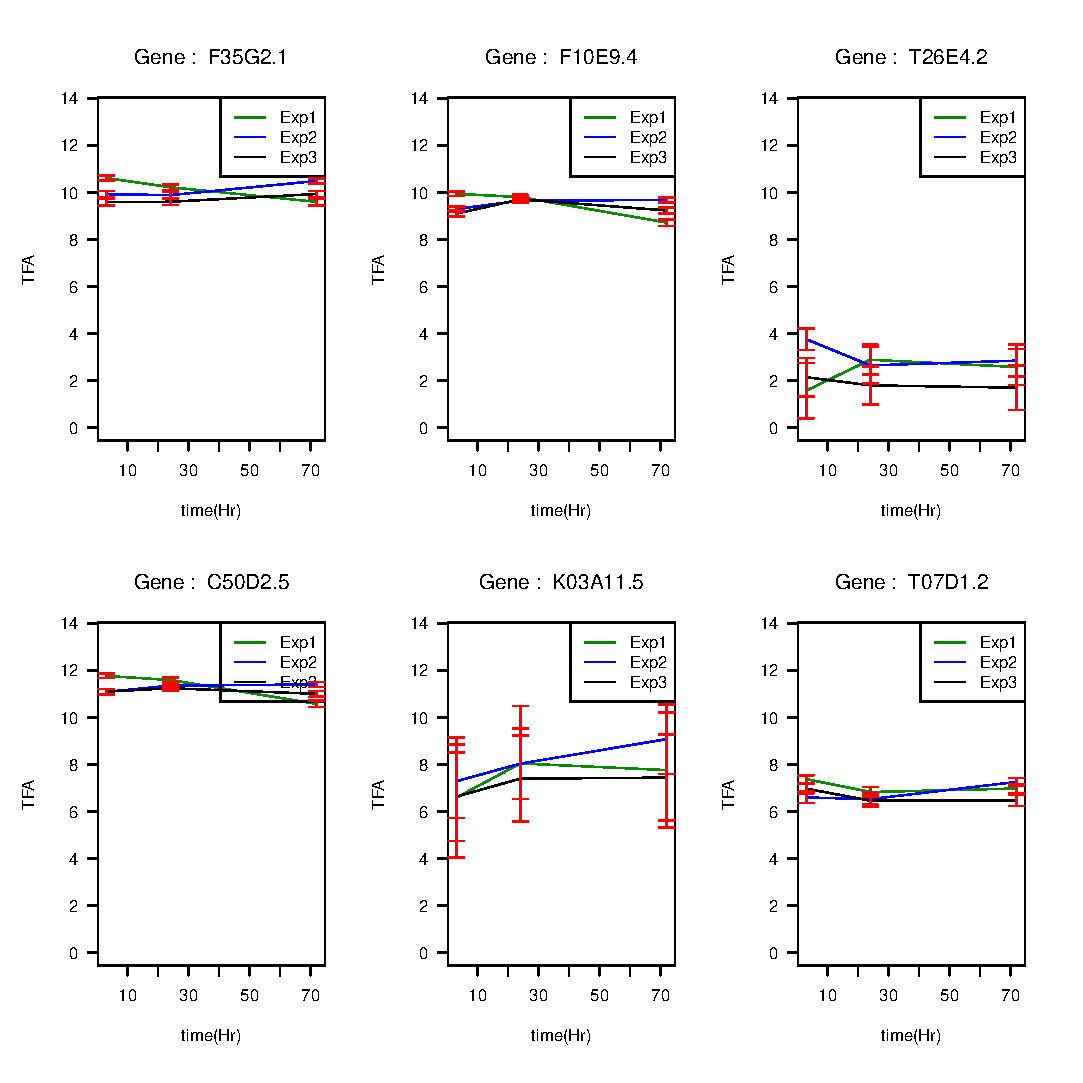
\includegraphics[width=1.0\linewidth]{picture/T20B12_8_3dp_CE_YH_tfid19.eps}
  \caption{Gene Specific TFA of T20B12.8}
  \label{fig:T20B12.8}
\end{figure}

      
Figure ~\ref{fig:F55D12.4} shows the transcription factor activity of F55D12.4 on F46A8.7
F55C9.11, R13A1.1, F10G8.6, Y106G6H.5 and Y71H2AM.5

\begin{figure}[!htb]
  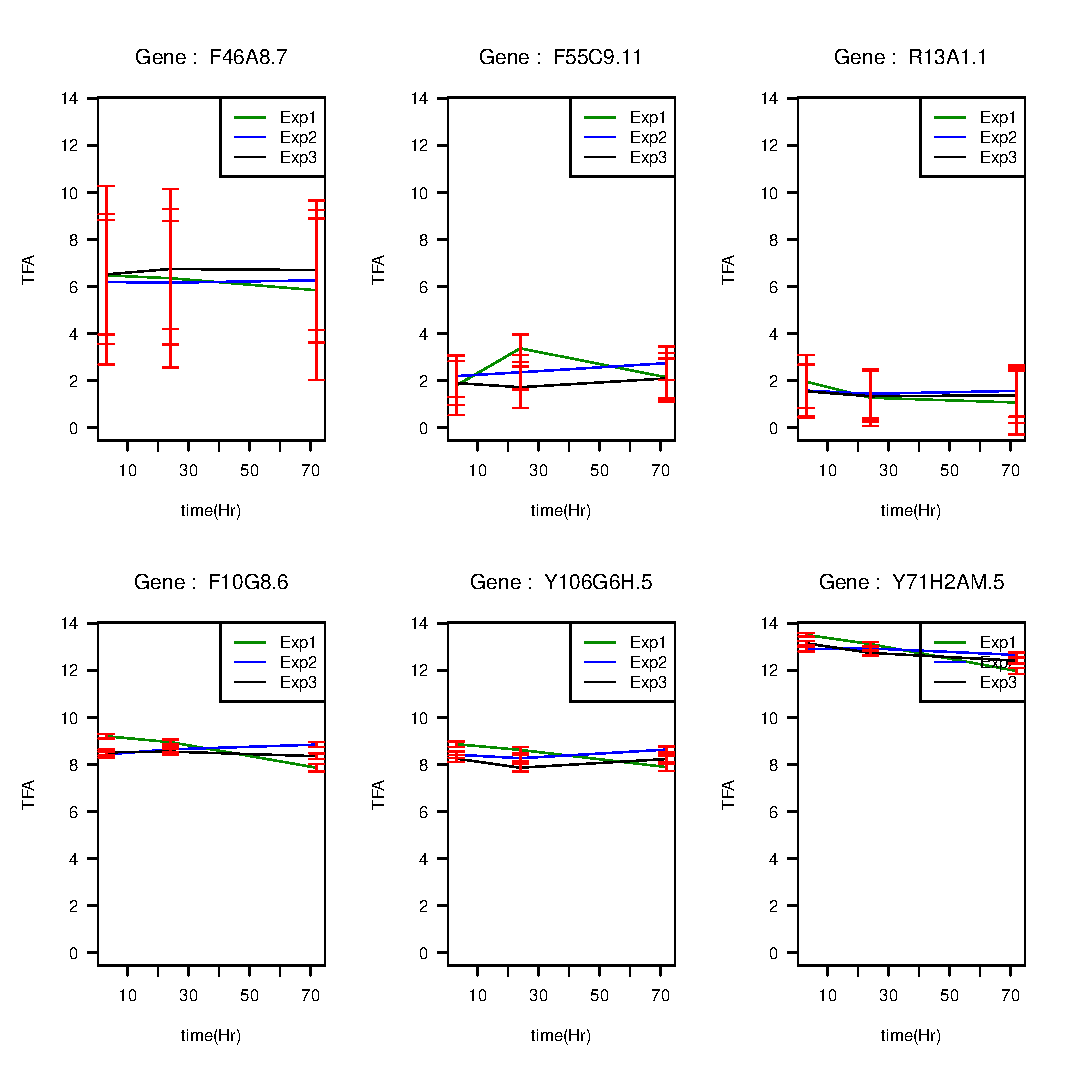
\includegraphics[width=1.0\linewidth]{picture/F55D12_4_3dp_HS_LC_tfid8.eps}
  \caption{Gene Specific TFA of F55D12.4}
  \label{fig:F55D12.4}
\end{figure}


\section{Key Questions}\label{conclusions}

\begin{itemize}
	\item Is there any specific gene (or set of genes) which dynamic TFA could be interesting?
	\item Are we interested to figure out the regulators activity for a certain gene?
	\item Is there any specific transcription factor which activity could be appealing?
	\item Whis relation of ~\cite{wormnet:url} is the right one to ontain the connectivity
	      between genes and transcription factors?
	\item We have only considered the common data from ~\cite{wormnet:url}, ~\cite{edgedb:01} 
	      and given data (from Andrew Cossins's lab). Is it OK? 
	\item For annotation and mapping between genes ID and ORF we have used ~\cite{celegans:db}.
	      Is it OK?
\end{itemize}	      
      
      

\section{Conclusions}\label{conclusions}

Have to write some conclusions


%\bibliographystyle{abbrv}
%\bibliographystyle{alpha}
\bibliographystyle{apalike}

\bibliography{bib_chipDyno}

\end{document}
